\documentclass[11pt, oneside]{article}   	% use "amsart" instead of "article" for AMSLaTeX format
\usepackage{geometry}                		% See geometry.pdf to learn the layout options. There are lots.
\geometry{letterpaper}                   		% ... or a4paper or a5paper or ... 
%\geometry{landscape}                		% Activate for for rotated page geometry
%\usepackage[parfill]{parskip}    		% Activate to begin paragraphs with an empty line rather than an indent
\usepackage{graphicx}				% Use pdf, png, jpg , or eps§ with pdflatex; use eps in DVI mode
								% TeX will automatically convert eps --> pdf in pdflatex		
\usepackage{amssymb}
\usepackage{amsmath}
\usepackage{parskip}
\usepackage{color}

\title{Kepler:  Area}
%\author{The Author}
%\section{}
% \subsection*{R code}
\date{}							% Activate to display a given date or no date

\graphicspath{{/Users/telliott_admin/Tex/png/}}

% \begin{center} 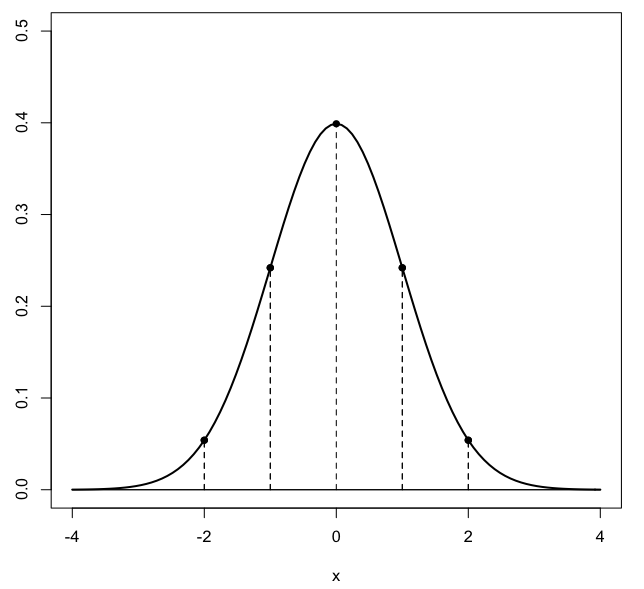
\includegraphics [scale=0.4] {gauss3.png} \end{center}

\begin{document}
\maketitle
\Large
\noindent

\subsection*{K2}

At this point, we have almost all the tools we need to follow the derivation of Kepler's law K2 ("equal areas in equal times") in Varberg \emph{Calculus} (online version, Chapter 14).  We just need a bit more discussion of area "swept out" by a planet in a short time.  

We revisit the triangle formed by the motion of the planet, and confirm that twice the area of the triangle is equal to
\[ h =  r^2 \ \frac{d \theta}{dt} \]
The thing that makes it confusing is that whereas Feynman used the velocity for one of the sides of the triangle and showed that
\[ \mathbf{r} \times \mathbf{v} = \mathbf{r} \times \dot{\mathbf{r}} = \mathbf{h}  \]
is a constant, Varberg use $d\mathbf{r}$ for their triangle.  

It leads to some confusing aspects in the presentation, which I want to work through since I like everything else about their derivation.  The bottom line is that before, when we referred to the change in area $\dot{A}$, we were really referring to the change in the change in area $\ddot{A} = 0$.

When Varberg talk about $A$, they really mean area, the total area since some particular start point.  Then $dA/dt = \dot{A}$ is the area swept out in a small unit of time, which is what we've previously called $A$.  So our previous $A$ is the same thing as what Varberg call $dA/dt$.  :)

Here is their diagram
\begin{center} 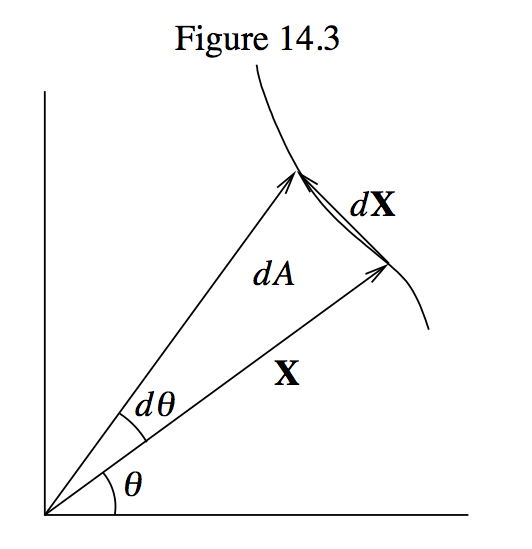
\includegraphics [scale=0.4] {Varberg14_3.png} \end{center}
They use $\mathbf{X}$ for the position vector, but I will label it as $\mathbf{r}$, following Feynman.  This vector "stays always in the $xy$-plane."  Also, I will use $\mathbf{u_r}$ for the vector they call $\mathbf{L}$ and similarly $\mathbf{u_\theta}$ for the vector they call $\mathbf{L}^{\perp}$.

We are asked to show that
\[ 2 \ \frac{dA}{dt} = \ | \frac{d\mathbf{r}}{dt} \times \mathbf{r} | \]

What I'm going to do is to change the notation a bit and say that in a short time $\Delta t$, the area that is swept out is $\Delta A$, corresponding to a length $d\mathbf{r} = \mathbf{v} \Delta t$, and that by the geometry we have
\[ 2 \ \Delta A = |\mathbf{r} \times \mathbf{v} \Delta t | \]
I assert that it is OK to bring $\Delta t$ out of the cross product (by the rule of scalar multiplication), since it is a scalar quantity, and is a constant at any stage of its future journey to the limit when $\Delta t \rightarrow 0$, so I write
\[ 2 \ \Delta A = |\mathbf{r} \times \mathbf{v} | \Delta t \]
Now we have 
\[ 2 \ \frac{\Delta A}{\Delta t} = |\mathbf{r} \times \mathbf{v} | \]
and in the limit
\[ 2 \ \frac{dA}{dt} = |\mathbf{r} \times \mathbf{v} | \]

Now this is not quite what we were asked to prove, but recall that
\[ \frac{d\mathbf{r}}{dt} \times \mathbf{r} = \dot{\mathbf{r}}  \times \mathbf{r} = - \mathbf{r} \times \dot{\mathbf{r}} \]
so the absolute values are the same.  Again, the result is that
\[ 2  \ \frac{dA}{dt} =  | \dot{\mathbf{r}} \times \mathbf{r} | = | \mathbf{r} \times \dot{\mathbf{r}} | = | \mathbf{h} | = h \]
If you're not completely happy with the argument allowing this step:
\[ 2 \ \Delta A = |\mathbf{r} \times \mathbf{v} \Delta t | = |\mathbf{r} \times \mathbf{v} | \Delta t \]
recall that 
\[ \mathbf{r} \times \mathbf{v} = \mathbf{r} \times \dot{\mathbf{r}} = \mathbf{h}  \]
so
\[ |\mathbf{r} \times \mathbf{v} \Delta t | = |\mathbf{c} \Delta t | = h \Delta t  \]

Varberg \emph{et al.} also give a second argument which which we will go through because it gives us the term
\[ r^2 \ \frac{d \theta}{dt} = h \]
By the geometry of the triangle, the area is
\[ 2 \ dA = r \ r d \theta = r^2 d \theta \]
where $r$ is $|\mathbf{r}|$.  And then they say
\[ 2 \ \frac{dA}{dt} = r^2 \ \frac{d\theta}{dt}  \]
They do this without comment, but this result assumes that $r$ does not vary with time, although clearly it does (that's the whole point of everything we are doing here).  The product rule would give us:
\[ \frac{d}{dt} \ r^2 d \theta = 2 r \ d \theta  \ \frac{dr}{dt} + r^2 \ \frac{d\theta}{dt}  \]

This looks a little weird because of the single differential $d\theta$, but what it means is that in the limit, the first term on the right-hand side goes to zero.

Another way of explaining this is to break the area into two parts.  
\begin{center} \includegraphics [scale=0.6] {kepler_area_calc.png} \end{center}
The first part is $(1/2) r$ times $r \ d\theta$, the length of (almost straight) arc perpendicular to $\mathbf{r}$.  This is the part we get by assuming that $r$ is constant.  And in the limit as $t \rightarrow 0$, the resulting $d\theta/dt$ has some value, namely, the angular velocity.

The second part is $(1/2) r \ d\theta$ times $dr$.  This is the part that accounts for the change in $r$, but it contains two differentials, only one of which gets rescued into some quantity by $dt$.  The other just goes to zero, so the whole thing is zero. 

Anyway, let's continue with the argument.

Go back to the right-hand side of what we were asked to prove above
\[ 2 \ \frac{dA}{dt} =  | \frac{d\mathbf{r}}{dt} \times \mathbf{r} | \]

and show that it turns into $r^2 d\theta/dt$.  Using $\mathbf{u_r}$ for the unit vector in the $\mathbf{r}$ direction, we have

\[ \frac{d\mathbf{r}}{dt}  = \frac{d}{dt} (r \mathbf{u_r}) = \frac{dr}{dt} \mathbf{u_r} + r \dot{\mathbf{u}}_\mathbf{r} \]

where the first part is just separating the scalar and unit vector part of $\mathbf{r}$ and the rest is from the product rule.  At this point we recall the result that $\dot{\mathbf{u}}_\mathbf{r}  = d \theta/dt \ \mathbf{u_\theta}$, so we have

\[ = \frac{dr}{dt} \mathbf{u_r} + r  \frac{d \theta}{dt} \ \mathbf{u_\theta} \]

So now this is what we need to cross with $\mathbf{r}$, also known as $r \mathbf{u_r}$.  We write

\[ (\frac{dr}{dt}  \mathbf{u_r} + r  \frac{d \theta}{dt} \  \mathbf{u_\theta}) \times r  \mathbf{u_r} \]
\[ = (\frac{dr}{dt}  \mathbf{u_r} \times  r  \mathbf{u_r}) + (r  \frac{d \theta}{dt} \  \mathbf{u_\theta} \times r  \mathbf{u_r}) \]

The first term is zero (the cross-product of $\mathbf{u_r}$ with itself), and because these are unit vectors the absolute value of the second term's vector cross-product is $1$

\[ | r  \frac{d \theta}{dt} \ \mathbf{u_\theta} \times r \mathbf{u_r} | =  r^2 \frac{d \theta}{dt} \ |  \mathbf{u_\theta} \times  \mathbf{u_r} | =  r^2 \frac{d \theta}{dt} \]

So what we've shown is that 

\[ 2 \ \frac{dA}{dt} =  | \mathbf{r} \times \dot{\mathbf{r}} | \]

and

\[ 2 \ \frac{dA}{dt} =  r^2 \ \frac{d \theta}{dt} \]

This term ($r^2 \ d\theta/dt$) is what Hartig calls $c$ and the other guys call $h$.  As the vector $\mathbf{h}$, it points in the $\hat{\mathbf{k}}$ direction and is the angular momentum but without the mass component.

\end{document}  